
\subsubsection{Vélo en roue libre}
\label{exo_velo_roue_libre}
	
	Un/e cycliste s’élance dans une descente en roue libre. Avec son équipement et son vélo, sa masse est de \SI{75}{\kilogram}. Alors qu’il/elle passe un point d’altitude \SI{1200}{\metre} sa vitesse est de \SI[per-mode = symbol]{50}{\kilo\metre\per\hour}. Exactement \SI{7}{\minute} plus tard, il/elle passe un point d’altitude \SI{950}{\metre} à vitesse de \SI[per-mode=symbol]{62}{\kilo\metre\per\hour}.
	
	\begin{enumerate}
		\item Quelle quantité d’énergie a-t-il/elle dissipée sous forme de frottements entre ces deux points ?
	\end{enumerate}
	
	Plus loin dans la descente, toujours en roue libre, le/la cycliste voit sa vitesse se stabiliser à \SI{45}{\kilo\metre\per\hour} dans une pente à \SI{4}{\percent}.
	
	\begin{enumerate}
		\shift{1}
		\item Avec quelle puissance dissipe-t-il/elle de l’énergie sous forme de frottements ?
	\end{enumerate}


\subsubsection{Refroidissement et puissance de centrale à vapeur}
\label{exo_refroidissement_centrale_vapeur}

	Le circuit suivi par l’eau dans les centrales à vapeur peut être représenté de façon simplifiée de la façon suivante (\cref{fig_cycle_rankine_chap_un}) :
	
			\begin{figure}
			\begin{center}
				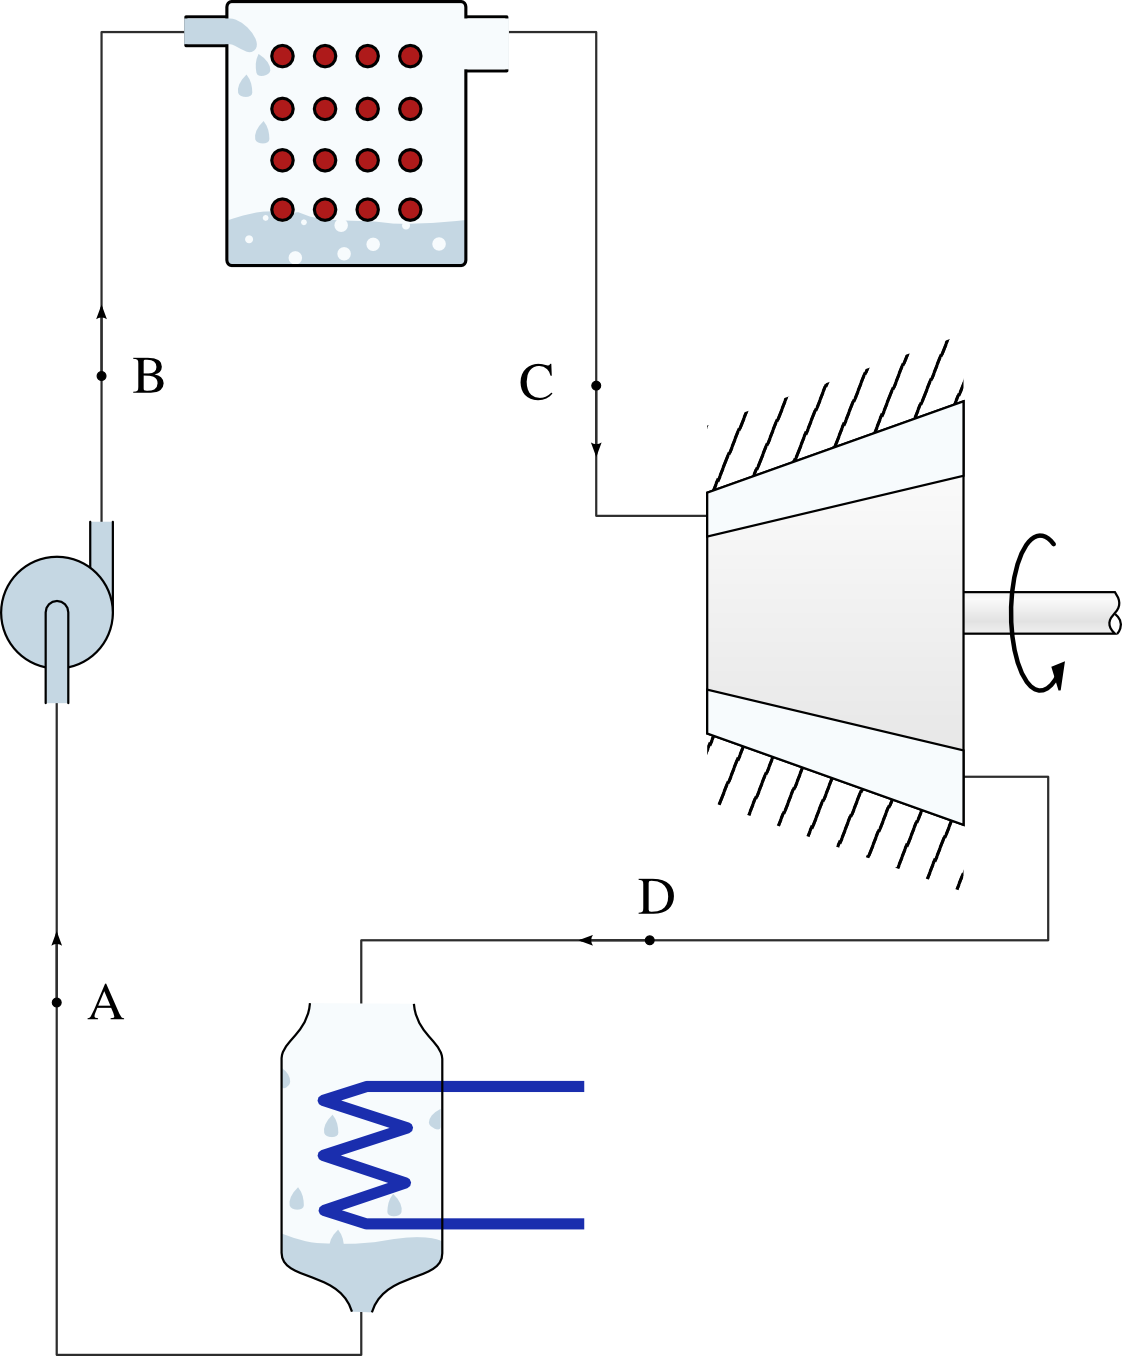
\includegraphics[height=11cm]{images/circuit_rankine.png}
			\end{center}
			\supercaption{Schéma simplifié du circuit suivi par l’eau à l’intérieur d’une centrale à vapeur. L’eau y suit un cycle complet en passant par quatre transformations. \\
			Ce circuit, nommé cycle de Rankine, est étudié de façon plus approfondie au \coursneuf (\cref{ch_cycle_de_rankine}).}{}
			\label{fig_cycle_rankine_chap_un}
		\end{figure}

		\begin{description}
			\item[De A à B] l’eau liquide est comprimée dans la pompe. Elle y reçoit un travail spécifique $w_\fromatob = \SI{+50}{\kilo\joule\per\kilogram}$, sans transfert de chaleur.
			\item[De B à C] l’eau est chauffée dans la chaudière d’où elle ressort sous forme de vapeur. Elle y reçoit une chaleur spéficique $q_\frombtoc = \SI{+450}{\kilo\joule\per\kilogram}$, sans recevoir de travail.
			\item[De C à D] l’eau se détend dans la turbine, où elle dégage un travail spécifique $w_\fromctod = \SI{-194}{\kilo\joule\per\kilogram}$, sans recevoir ou perdre de chaleur.
			\item[De D à A] l’eau est refroidie dans un condenseur, sans transfert de travail, où elle retrouve son état et ses propriétés originaux, avant de retourner à la pompe pour être à nouveau comprimée.
		\end{description}

	Le débit d’eau circulant dans l’installation est de \SI{15}{\kilogram\per\second}.

	\begin{enumerate}
		\item Quelle est la puissance spécifique rejetée sous forme de chaleur dans le condenseur ?
		\item Quelle est la puissance (en \si{watts}) rejetée par le condenseur ?
		\item Quelle est la puissance (en \si{watts}) dégagée par la turbine sous forme de travail ?
		\item Quelle est l’efficacité $\eta_{\text{centrale}}$ de la centrale, c’est à dire le rapport entre sa puissance nette et sa consommation brute ?
	\end{enumerate}	

\subsubsection{Compression de ressorts}
\label{exo_compression_ressorts}
	
	Dans le laboratoire d’une entreprise fabriquant des systèmes de suspension automobile, un/e ingénieur/e compare les caractéristiques de trois ressorts de géométrie différente. Pour cela il/elle mesure la force $F$ (en \si{\newton}) exercée par chaque ressort en fonction de sa longueur $l$ (en~\si{\metre}), et modélise ces comportements ainsi :
	
		\begin{itemize}
			\item \onlyframabook{~~}$F_{\A\ (l)} = \num{8e3} - \num{2e3} \ l$
			\item \onlyframabook{~~}$F_{\B\ (l)} = \num{8e3} - \num{3e3} \ l^{\num{1,6}}$
			\item \onlyframabook{~~}$F_{\C\ (l)} = \num{0,1e3} \ l^{\num{-3}}$
		\end{itemize}
		
	Quelle est la quantité de travail qu’il faut fournir à chacun de ces ressorts pour les comprimer depuis une longueur de \SI{40}{\centi\metre} jusqu’à une longueur de \SI{12}{\centi\metre} ?
	
	Nous verrons au \coursdeux que lorsque les fluides sont comprimés et détendus lentement, ils se comportent de façon similaire au ressort C, de géométrie conique comme ceux représentés en \cref{fig_ressorts_coniques}.
	
	\begin{figure}
		\begin{center}
			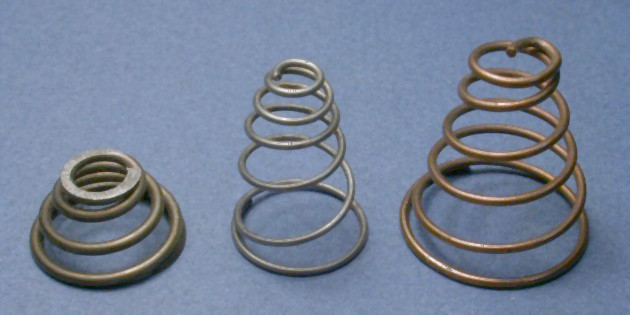
\includegraphics[width=0.6\textwidth]{images/ressorts_coniques.jpg}
		\end{center}
		\supercaption{Ressorts coniques, dont la dureté augmente exponentiellement lorsqu’on les comprime.}{\wcfile{Ressorts_de_compression_coniques.jpg}{Photo} \ccbysa Jean-Jacques Milan}
		\label{fig_ressorts_coniques}
	\end{figure}
	

\subsubsection{Moteur à ressorts}
\label{exo_ressorts_moteur}

	\wherefrom{[dér. DS n°1 2012 7pts]}
	
	Nous modélisons le fonctionnement d’un moteur à essence en remplaçant l’air dans un cylindre par un ressort. Nous voulons quantifier l’énergie emmagasinée puis perdue par un ressort puissant pendant un aller-retour (comme l’air pendant les phases de compression et de détente d’un cycle moteur).

	\begin{figure}
	\begin{center}
		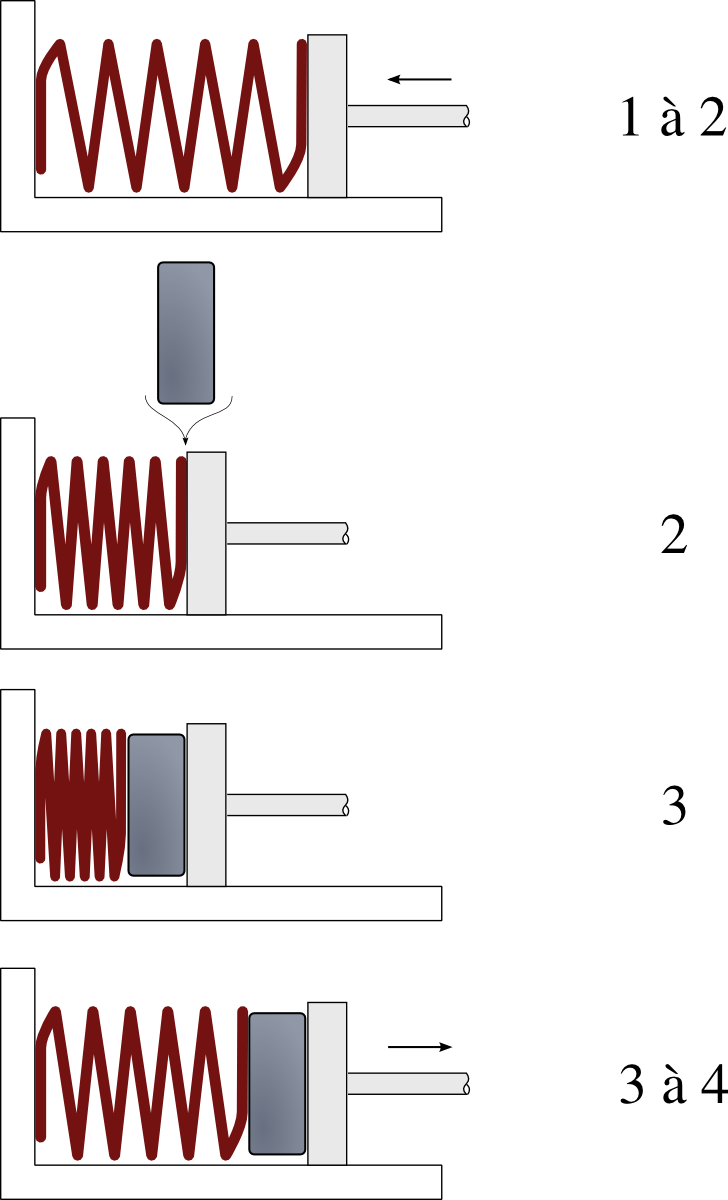
\includegraphics[width=0.5\textwidth]{images/piston_ressorts.png}
	\end{center}
	\caption{Expérience réalisée avec un ressort puissant. Le piston écrase le ressort de $1$ à $2$, puis le ressort repousse le piston de $3$ à $4$. Au retour, la force exercée par le ressort est plus grande.}
	\label{fig_pistons_ressorts}
	\end{figure}

	L’expérience se déroule de façon cyclique avec les quatre étapes suivantes (\cref{fig_pistons_ressorts}) :
	
	\begin{description}
		\item[De 1 à 2 :] L’expérimentateur comprime un ressort depuis une longueur de~\SI{25}{\centi\metre} vers une longueur de~\SI{8}{\centi\metre}.
		Le ressort exerce une force liée à sa longueur (en mètres) par la relation :
		
		\begin{equation}
			F = \num{25,4e3} - \num{40e3} \ l
		\end{equation}
		
		\begin{description}
			\item où $F$ est la force (\si{\newton}) ;
			\item et $l$ est la longueur du ressort (\si{\metre}).
		\end{description}

		\item[De 2 à 3 :] Lorsque la longueur du ressort arrive à~\SI{8}{\centi\metre}, l’expérimentateur bloque le déplacement du piston. Un bloc solide est alors inséré entre la paroi du piston et le ressort. \\
		La force sur le piston (qui n’a pas bougé) augmente jusqu’à atteindre \SI{32}{\kilo\newton}.
		
		\item[De 3 à 4 :] Une fois que le bloc a été inséré, l’expérimentateur effectue le chemin du retour avec le piston, jusqu’à ce que la longueur finale atteigne à nouveau \SI{25}{\centi\metre}.
		
		\item[De 4 à~1 :] On retire le bloc sans déplacer le piston, et la force sur le piston revient à la valeur qu’elle avait au début de l’expérience.
	\end{description}
	
	Nous souhaitons quantifier l’énergie emmagasinée puis perdue par l’ensemble \{ressort+bloc\} pendant un aller-retour. 
	
	\begin{enumerate}
		\item Représentez l’évolution sur un diagramme montrant la force en fonction de la longueur à l’intérieur, de façon qualitative (c’est-à-dire sans représenter les valeurs numériques).
		\item Combien d’énergie le ressort a-t-il reçu de l’expérimentateur pendant le chemin aller (de 1 à 2) ?
		\item Quelle est la caractéristique $F_{(l)}$ de l’ensemble \{ressort+bloc\} pendant le chemin de retour (de~3 à~4) ?
		\item Combien d’énergie le ressort a-t-il reçu du piston pendant le chemin retour (de~3 à~4) ?
		\item Au final, combien d’énergie l’expérimentateur a-t-il reçu ou dépensé pendant l’expé\-rience ?
		\item Avec quelle fréquence doit-t-il répéter l’expérience pour que la puissance atteigne \SI{25}{ch}, c’est-à-dire \SI{18,4}{\kilo\watt} ?
	\end{enumerate}


\subsubsection{Préparation d’un bain}
\label{exo_bain}

	Un/e étudiant/e épuisé/e par le calcul intégral de compression de ressorts souhaite prendre un bain. 
	
	L’eau courante arrive à température de~\SI{10}{\degreeCelsius} dans le chauffe-eau électrique ; elle a une capacité calorifique constante de~$c_{\text{eau liquide}} = \SI{4,2}{\kilo\joule\per\kilogram\per\kelvin}$ et une masse volumique constante $\rho_{\text{eau liquide}} = \SI{e3}{\kilogram\per\metre\cubed}$.
	
	\begin{enumerate}
		\item Combien faut-il d’énergie pour chauffer l’eau à \SI{40}{\degreeCelsius} afin de remplir une baignoire de~\SI{270}{\liter} ?
		\item Combien de temps le réchauffage prendra-t-il si la puissance de chauffage est de~$\dot Q = \SI{+2}{\kilo\watt}$ ?
	\end{enumerate}



\subsubsection{Cric hydraulique}
\label{exo_cric}

	\wherefrom{[DS n°1 2012, 5pts]}

	On souhaite lever un véhicule ayant pour masse \SI{1200}{\kilogram} avec le cric hydraulique schématisé en \cref{fig_cric}. Le piston gauche a pour surface \SI{5}{\centi\metre\squared}.	

	\begin{figure}
		\begin{center}
			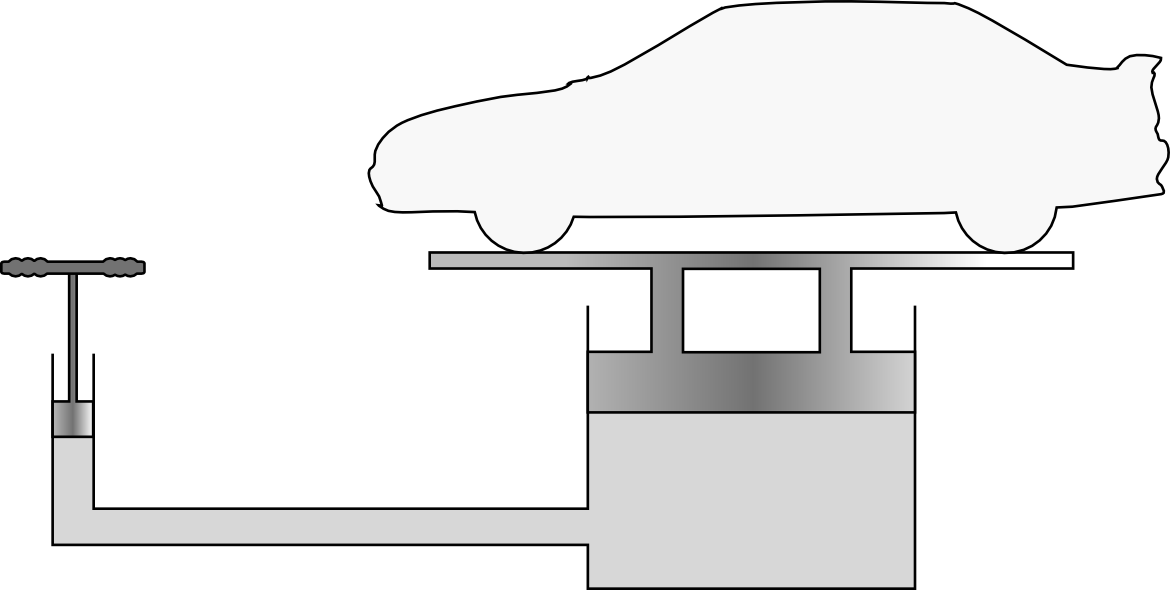
\includegraphics[width=12cm]{images/cric.png}
		\end{center}
		\caption{Schéma de principe d’un cric hydraulique.}
		\label{fig_cric}
	\end{figure}

	L’huile au sein du cric est présumée incompressible, c’est-à-dire que son volume est considéré comme constant quelle que soit la pression. 

	Le but de l’installation est de permettre à une personne de gabarit ordinaire de soulever et maintenir en place le véhicule avec le piston gauche (dont l’extrémité est munie de poignées).
	
		\begin{enumerate}
			\item Dimensionnez le piston droit (sous le véhicule) afin que la force dans le piston gauche n’excède pas \SI{100}{\newton}.
			\item Quelle est la puissance nécessaire pour maintenir le véhicule en place ?
		\end{enumerate}
	On souhaite soulever le véhicule de~\SI{25}{\centi\metre}, en moins de 30 secondes.
		\begin{enumerate}
			\setcounter{enumi}{2}
			\item Selon quelle distance faudrait-t-il enfoncer le piston gauche pour cela ?
			\item Quels seraient alors le travail et la puissance à fournir ?
		\end{enumerate}


\subsubsection{Turbine à eau}
\label{exo_turbine_eau_puissances_spe}
	
	Un débit constant de \SI{1200}{\kilogram\per\second} traverse une petite installation hydraulique représentée en \cref{fig_turbine_hydraulique_exo}.
	\begin{itemize}
		\item Au point $1$, l’eau arrive à vitesse de \SI{3}{\metre\per\second} avec une température $T_1 = \SI{5}{\degreeCelsius}$ et une altitude $z_1 = \SI{75}{\metre}$. 
		\item Au point $2$, elle ressort à vitesse de \SI{2,5}{\metre\per\second} à température $T_2 = \SI{5,04}{\degreeCelsius}$ et altitude $z_2 = \SI{4}{\metre}$.
	\end{itemize}

	\begin{figure}
		\begin{center}
			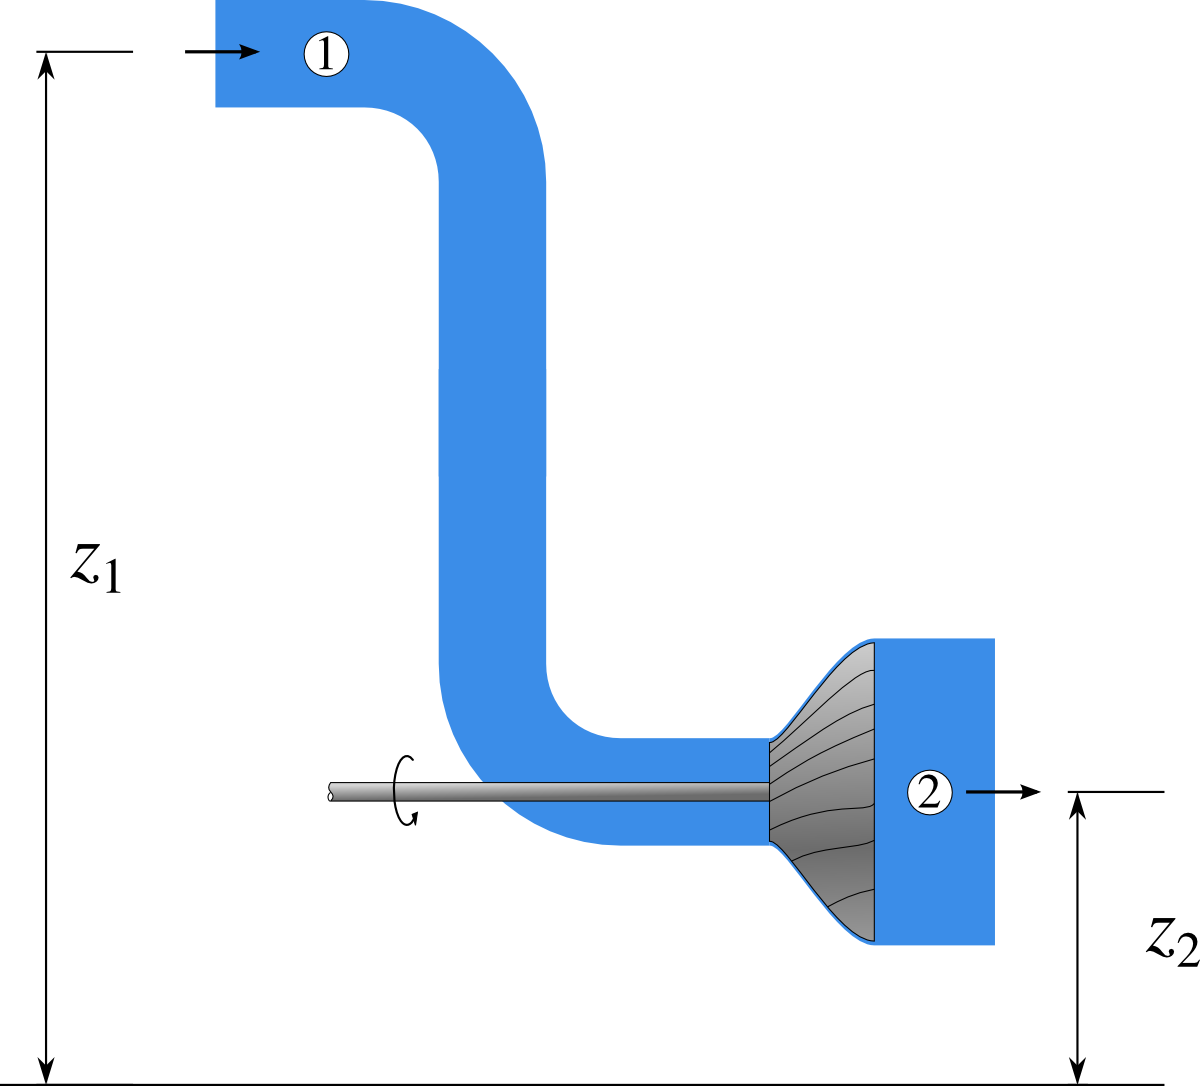
\includegraphics[width=0.6\textwidth]{images/turbine_eau.png}
		\end{center}
		\caption{Schéma de principe d’une turbine à eau. L’eau pénètre en haut à gauche, fait tourner les pales de la turbine, est réchauffée par frottement, et ressort en bas à droite de l’installation.}
		\label{fig_turbine_hydraulique_exo}
	\end{figure}
	
	La pression de l’eau est identique en 1 et 2, et le profil de vitesse de l’eau en chaque point est approximativement uniforme. L’eau a une capacité calorifique massique de $c_{\text{eau liquide}} = \SI{4,2}{\kilo\joule\per\kilogram\per\kelvin}$.
	
	\begin{enumerate}
		\item Quelle est la puissance spécifique mécanique gagnée ou perdue par l’eau en traversant l’installation ?
		\item Avec quelle puissance spécifique est-elle réchauffée par le frottement ?
		\item Quelle est la puissance (en \si{watts}) dégagée sous forme de travail par la turbine ?
	\end{enumerate}


\subsubsection{Chaudière de chauffage central}
\label{exo_chaudiere_simple}

	La chaudière du système de chauffage central d’un bâtiment, représenté en \cref{fig_chaudiere_eau}, fonctionne avec la combustion du kérosène.

	\begin{figure}
		\begin{center}
			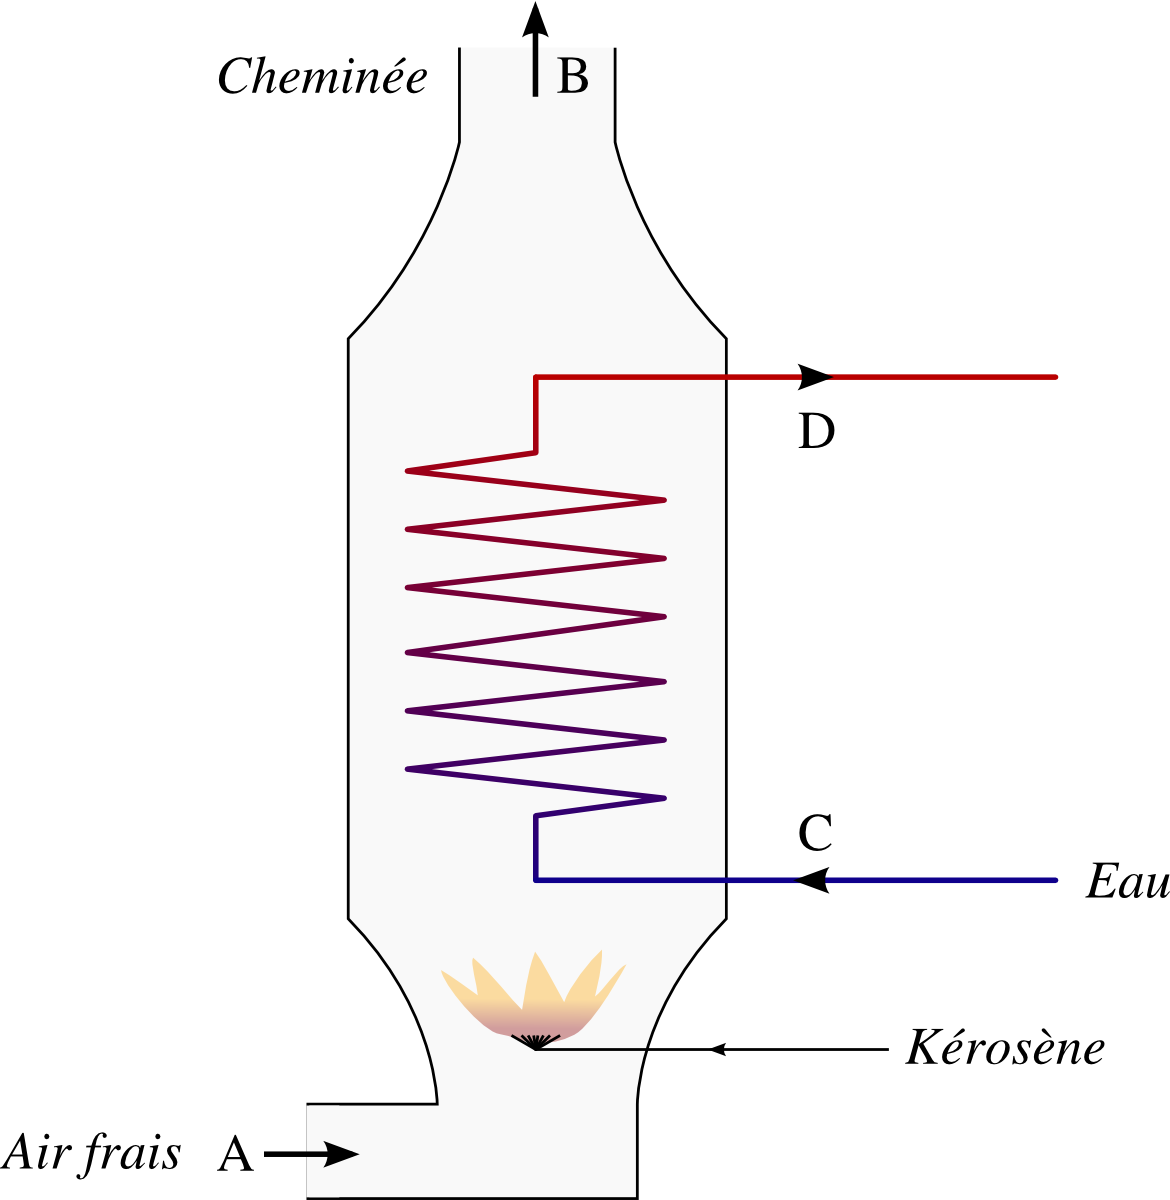
\includegraphics[width=0.7\textwidth]{images/chaudiere_eau.png}
		\end{center}
		\caption{Schéma de principe d’une chaudière utilisée pour le chauffage d’un bâtiment. L’eau ($\C \to D$) y pénètre par la droite, et y est réchauffée par l’air ($\A \to \B$) mélangé au kérosène.}
		\label{fig_chaudiere_eau}
	\end{figure}
	
	L’eau pénètre dans la chaudière à une température $T_\C = \SI{20}{\degreeCelsius}$ et en ressort à $T_\D = \SI{70}{\degreeCelsius}$, avec un débit $\dot V_{\text{eau}} = \SI{0,25}{\liter\per\second}$.
	
	La chambre de combustion admet de l’air à~$T_\A = \SI{8}{\degreeCelsius}$ et il ressort par la cheminée à une température $T_\B = \SI{120}{\degreeCelsius}$ ; le débit d’air est de~$\dot m_{\text{air}} = \SI{0,5}{\kilogram\per\second}$.
	
	\TabPositions{11cm}
	Chaleur spécifique de combustion du kérosène  : 			\tab \SI{46,4}{\mega\joule\per\kilogram}
	
	Capacité calorifique massique de l’eau liquide  : 			\tab \SI{4,18}{\kilo\joule\per\kilogram\per\kelvin}
	
	Capacité calorifique massique de l’air à pression constante  : 	\tab \SI{1,15}{\kilo\joule\per\kilogram\per\kelvin}
	\TabPositions{6cm} % back to default

	\begin{enumerate}
	\item Quelle est la consommation horaire de kérosène par la chaudière ?
	\item Quelle est l’efficacité de la chaudière, c’est à dire le rapport entre son transfert de chaleur utile et sa consommation énergétique ?
	\end{enumerate}


\subsubsection{Turbomoteur d’hélicoptère}
\label{exo_turbomoteur_puissances_spe}

	Un hélicoptère est muni de deux turbomoteurs, c’est à dire de turbomachines dont le but est de faire tourner un arbre sortant du moteur (\cref{fig_s76b}). Nous pouvons évaluer plusieurs caractéristiques de ces moteurs sans connaître précisément leur fonctionnement interne.
	
	Chacun des deux moteurs admet de l’air atmosphérique à température de \SI{15}{\degreeCelsius}. L’air y est compressé, réchauffé, puis détendu, ce qui permet de dégager du travail pour faire tourner les rotors. À la sortie du moteur, l’air est rejeté à pression atmosphérique et température de~\SI{360}{\degreeCelsius}.

	\begin{figure}
		\begin{center}
			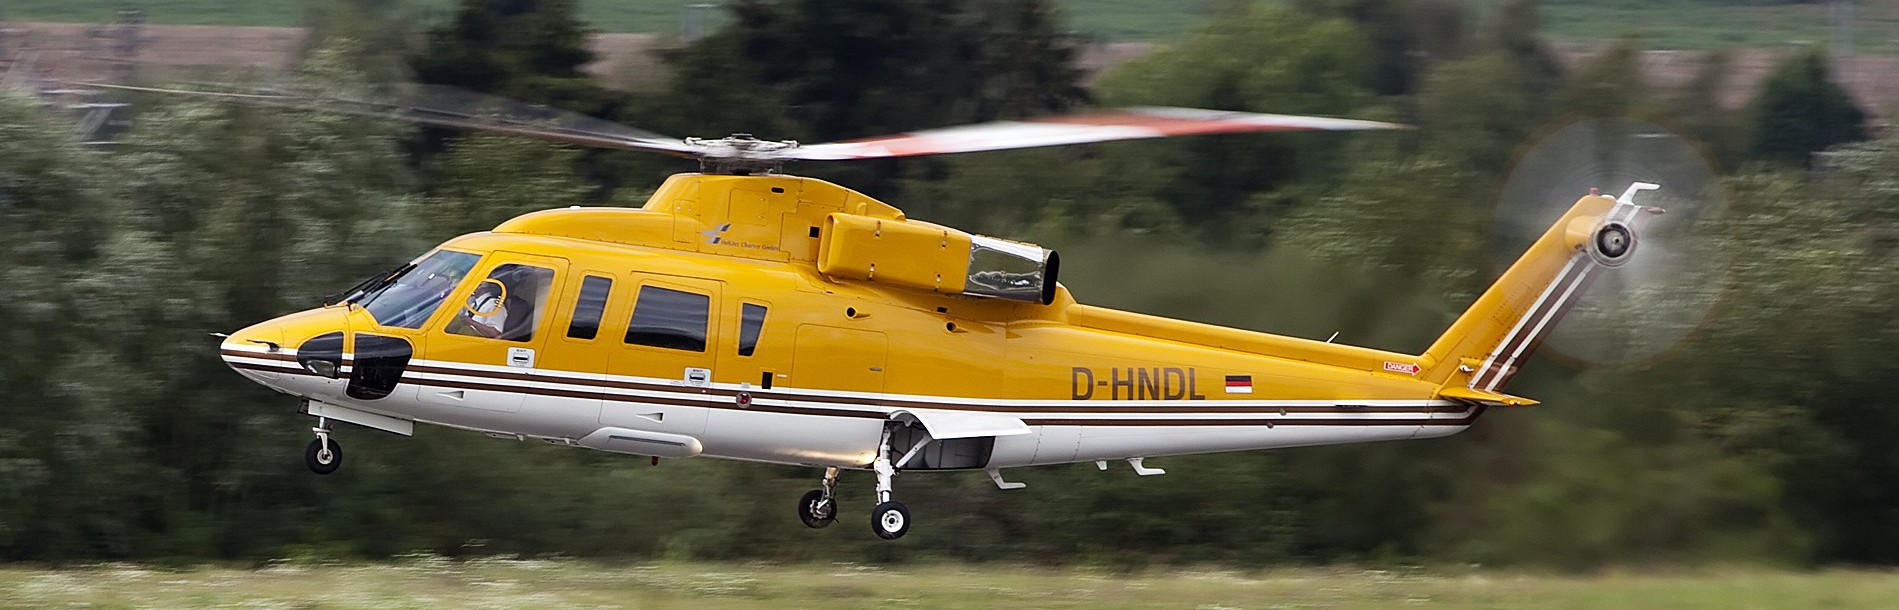
\includegraphics[width=0.8\textwidth]{images/sikorsky_s76b.jpg}
			\vspace{0.5cm}\\
			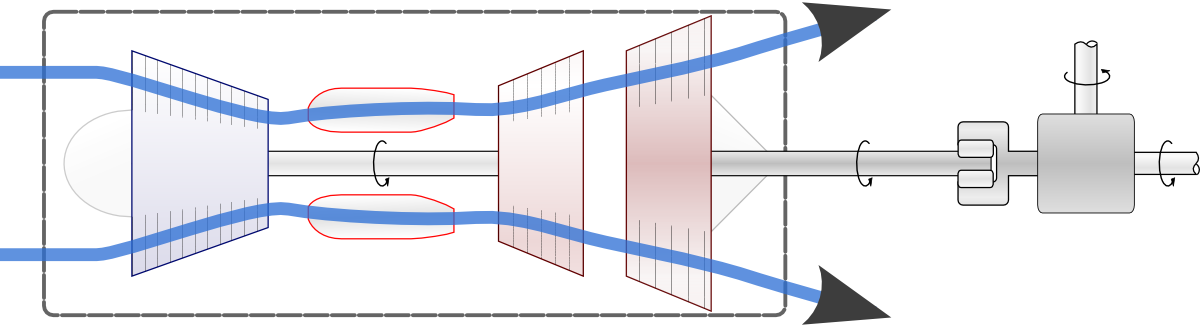
\includegraphics[width=0.8\textwidth]{images/turbomoteur_principe.png}
		\end{center}
		\supercaption{Un hélicoptère \wfd{Sikorsky S-76}{Sikorsky S-76B}, équipé de deux turbomoteurs \textit{P\&WC} \textsc{pt-6b} de \SI{980}{ch} chacun. Le trajet de l’air dans les moteurs est représenté dans un schéma de principe. Nous étudions ces moteurs plus en détail au \coursdix.}{\wcfile{D-HNDL_S76B_(6104005164).jpg}{Photo hélicoptère} \ccbysa Maarten Visser\\ Schéma \ccbysa \olivier}
		\label{fig_s76b}
	\end{figure}

	À pression constante, la capacité calorifique massique de l’air est environ $c_{p\ \text{air}} = \SI{1050}{\joule\per\kilogram\per\kelvin}$. La combustion du kérosène dégage $q_{\text{kérosène}} = \SI{46}{\mega\joule\per\kilogram}$.

	\begin{enumerate}
		\item Quelle est la puissance spécifique rejetée par le moteur dans l’atmosphère ?\\
			\footnotesize{Indice : c’est la chaleur spécifique que doit perdre l’air rejeté pour retrouver sa température initiale.}
	\end{enumerate}

	Le manuel de vol indique que dans la chambre de combustion (la partie du moteur où est brûlé le carburant), l’air est admis à température de \SI{250}{\degreeCelsius} et qu’il y est réchauffé par la combustion, à pression constante, jusqu’à~\SI{776}{\degreeCelsius}.
	
	\begin{enumerate}
		\shift{1}
		\item Quelle est la puissance spécifique dégagée par le moteur sous forme de travail ?\\
			\footnotesize{Indice : au final, toute l’énergie perdue par l’air sous forme de travail et de chaleur lui a été apportée dans la chambre de combustion.}
	\end{enumerate}
		
	Pour maintenir l’hélicoptère en vol stationnaire en pleine charge, les rotors demandent à chaque moteur une puissance sous forme de travail de \SI{900}{ch} (\SI{662}{\kilo\watt}).
	
	\begin{enumerate}
		\shift{2}
		\item Quel débit d’air faut-il admettre dans chaque turbomoteur ?
		\item Quelle est alors la puissance (en \si{\watt}) à fournir dans chaque chambre de combustion ?
		\item Quelle est la consommation horaire de kérosène en vol stationnaire ?
	\end{enumerate}

\exercisesolutionpage
\titreresultats

\begin{description}
	\item[\ref{exo_velo_roue_libre}] 
				\tab 1) $E_{\text{méca}2} - E_{\text{méca}1} = \SI{-180}{\kilo\joule}$ (le temps de \SI{7}{\minute} n’ayant bien sûr pas d’importance) 
				\tab 2) $\dot Q_{\text{frottements}} = m \ g \ \dot z = \SI{36,8}{\watt}$.
	\item[\ref{exo_refroidissement_centrale_vapeur}] 	
				\tab 1) Au final, l’eau a perdu autant d’énergie qu’elle en a reçu, donc $q_{\D \to \A} = - w_\fromatob - q_\frombtoc - w_\fromctod = \SI{-306}{\kilo\joule\per\kilogram} $ Nous avons fait fonctionner des moteurs pendant quarante ans avant de comprendre cela !
				\tab 2) $\dot Q_\fromdtoa = \dot m q_\fromdtoa = \SI{-4,59}{\mega\watt}$
				\tab 3) $\dot W_\fromctod = \dot m w_\fromctod = \SI{-2,91}{\mega\watt}$
				\tab 4) $\eta_{\text{centrale}} = \left|\frac{w_{\text{turbine}} + w_{\text{pompe}}}{q_{\text{chaudière}}}\right| = \SI{32}{\percent}$ (valeur réaliste).
	\item [\ref{exo_compression_ressorts}]
				\tab 1) $W_\A = \int_{l_1}^{l_2} F_{(l)} \diff l = - \num{e3} \left[ 8 l - \frac{1}{2} 2 l^2 \right]_{0,4}^{0,12} = \SI{+2,094}{\kilo\joule}$.
				\tab 2) $W_\B = \SI{+2,138}{\kilo\joule}$ 
				\tab 3) $W_\C = \SI{+3,157}{\kilo\joule}$.
	\item [\ref{exo_ressorts_moteur}] 
				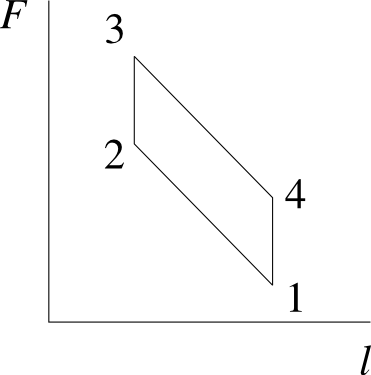
\includegraphics[width=\solutiondiagramwidth]{images/exo_sol_fl_ressorts_moteur.png}
				\tab 2) $W_{1 \to 2} = \SI{+3,179}{\kilo\joule}$ 
				\tab 3) $F_{(l) 3 \to 4} = \num{35,2e3} - \num{40e3} l$
				\tab 4) $W_{3 \to 4} = \SI{-4,862}{\kilo\joule}$
				\tab 5) $W_{\text{cycle}} = \SI{1,683}{\kilo\joule}$
				\tab 6) $f = \SI{10,9}{\per\second}$ (11 fois par seconde)
	\item [\ref{exo_bain}]
				\tab 1) $Q_{\text{eau}} = \rho_{\text{eau}} V_{\text{eau}} c_{\text{eau}} \Delta T = \SI{+30,24}{\mega\joule}$ 
				\tab 2) $\Delta t = \frac{Q_{\text{eau}}}{\dot Q} = \SI{4,2}{\hour}$
	\item [\ref{exo_cric}] 	
				\tab 1) $S_2 \leq \frac{F_2}{p_2} = \frac{F_2}{p_1} = \SI{5,89e-2}{\metre\squared} = \SI{589}{\centi\metre\squared}$
				\tab 2) $\dot W = \SI{0}{\watt}$ bien sûr, puisqu’il n’y a pas de déplacement\ldots
				\tab 3) En calculant le volume $V$ d’huile balayé, $d_1 = \frac{V_1}{S_1} = \frac{V_2}{S_2} = \SI{29,43}{\metre}$, une longueur impraticable sans ajouter un mécanisme de pompage.
				\tab 4) $\dot W_{\text{moyen}} \leq \frac{W_\fromatob}{\Delta t} = \SI{98,1}{\watt}$.
	\item [\ref{exo_turbine_eau_puissances_spe}]
				\tab 1) $\Delta e_{\text{méca.}} = \SI{-697,9}{\joule\per\kilogram}$ (donc une perte par l’eau)
				\tab 2) $q_{1 \to 2} = \SI{+168}{\joule\per\kilogram}$
				\tab 3) $\dot W_{\text{turbine}} = \dot m (\Delta e_{\text{méca.}} + q_{1 \to 2} ) = \SI{-635,9}{\kilo\watt}$.
	\item [\ref{exo_chaudiere_simple}] 	
				\tab 1) $\dot m_{\text{kérosène}} = \frac{\dot Q_{\text{kérosène}}}{q_{\text{kérosène}}} = \frac{-\dot Q_{\text{eau}} - \dot Q_{\text{air}}}{q_{\text{kérosène}}} =  \SI{2,51e-3}{\kilogram\per\second} = \SI{9,1}{\kilogram\per\hour}	$
				\tab 2) $\eta_{\text{chaudière}} = \left|\frac{\dot Q_{\text{eau}}}{\dot Q_{\text{kérosène}}}\right| = \SI{44,8}{\percent}$
	\item [\ref{exo_turbomoteur_puissances_spe}]
				\tab 1) $q_{\text{rejet}} = \SI{+362,25}{\kilo\joule\per\kilogram}$
				\tab 2) $q_{\text{chambre}} + w_{\text{arbre}} + q_{\text{refroidissement atmosphérique}} = 0$ ou encore $q_{\text{chambre}} + w_{\text{arbre}} - q_{\text{rejet}} = 0$ ; ainsi on a $w_{\text{arbre}} = - q_{\text{chambre}} + q_{\text{rejet}} = \SI{-361,7}{\kilo\joule\per\kilogram}$.
				\tab 3) $\dot m_{\text{air}} = \SI{1,83}{\kilogram\per\second}$
				\tab 4) $\dot Q_{\text{chambre}} = \SI{1,011}{\mega\watt}$
				\tab 5) $\dot m_{\text{kérosène}} = 2 \frac{\dot Q_{\text{chambre}}}{q_{\text{kérosène}}} = \SI{158,2}{\kilogram\per\hour}$ (valeur sensiblement plus faible que la réalité).
\end{description}

